\documentclass[12pt]{article}

\usepackage[margin = .8in]{geometry}
\usepackage{amsmath}
\usepackage{graphicx}
\usepackage{multicol, enumerate}

\usepackage{fancyhdr}
\pagestyle{fancy}

\lhead{Math F113X: Numbers and Society}
\rhead{Date: \hspace{1in}}

\usepackage{tikz}
\usetikzlibrary{calc,trees,positioning,arrows,fit,shapes,through}
\usetikzlibrary{patterns}

\usetikzlibrary{decorations.markings}
\usetikzlibrary{arrows}

\usepackage{pgfplots}

\usepackage{longtable}
\usepackage{tabularx}

\newcommand{\ds}{\displaystyle}
\newcommand{\ans}[1][1in]{\rule{#1}{.5pt}}

\newcommand{\points}[1]{(#1 points.)}		% Trying to be lazy.

\usepackage{array}
\newcolumntype{L}[1]{>{\raggedright\let\newline\\\arraybackslash\hspace{0pt}}m{#1}}
\newcolumntype{C}[1]{>{\centering\let\newline\\\arraybackslash\hspace{0pt}}m{#1}}
\newcolumntype{R}[1]{>{\raggedleft\let\newline\\\arraybackslash\hspace{0pt}}m{#1}}
\newcommand{\red}[1]{\textcolor{red}{#1}}

\newcommand{\be}{\begin{enumerate}}
\newcommand{\ee}{\end{enumerate}}

%\topmargin -1in
%\textheight 9.5in
%\oddsidemargin -0.3in
%\evensidemargin \oddsidemargin
%\pagestyle{empty}
%%\marginparwidth 0.5in
%\textwidth 7in
%\parindent 0in

%--------------------------------------------------------------------------------------------------------------------------------------------------------------------------
%						Document
%--------------------------------------------------------------------------------------------------------------------------------------------------------------------------


\begin{document}
%\pagestyle{fancy}
\begin{center}
{\Large  Worksheet 9 (Graph Theory 1): Pieces of Graphs}
\end{center}



\noindent \textbf{Group Names:} \hrulefill \\
%-------------------------------------------------------------------------------------------------------------
%						Assignment
%-----------------------------------------------------------------------------------------------------
\begin{enumerate}
\item Graph $Q$ is shown below (twice). Answer the questions:


%\begin{minipage}{.4\linewidth}
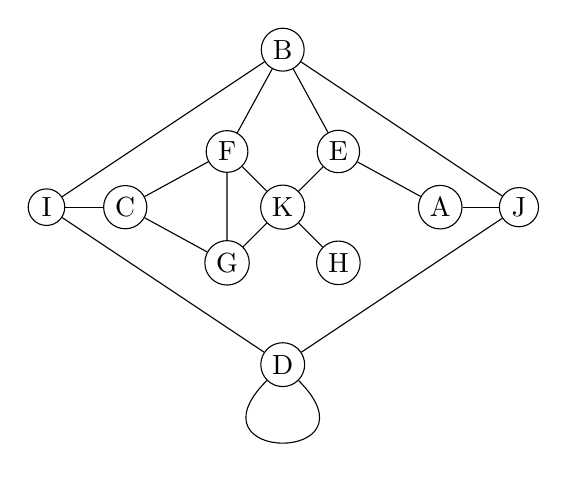
\begin{tikzpicture}[vertex/.style={circle, draw, inner sep=2pt}, every node/.style={vertex}]%, minimum size=6pt]

%\tikzstyle{every node} = [vertex];
\node (A) at (0:2) {A};
\node (B) at (90:2) {B};
\node (C) at (180:2) {C};
\node (D) at (270:2) {D};
\node (O) at (0,0){K};
\node (E) at (45:1) {E};
\node (F) at (45+90:1){F};
\node (G) at (45+180:1){G};
\node (H) at (45+270:1){H};
\node[left of = C] (I) {I};
\node [right of = A] (J) {J};
\draw (D) to[out = 270-45, in = 270+45, distance = 1.5cm] (D);
\draw (B) -- (I) -- (D) -- (J)--(B);
\draw (A) -- (E) -- (B) -- (F) -- (C) -- (G);% -- (D) -- (H) -- (A);
\draw (E) -- (O) -- (G)-- (F) --(O) --(H);
\draw (A) -- (J) (C) -- (I);
\end{tikzpicture}
\hfill
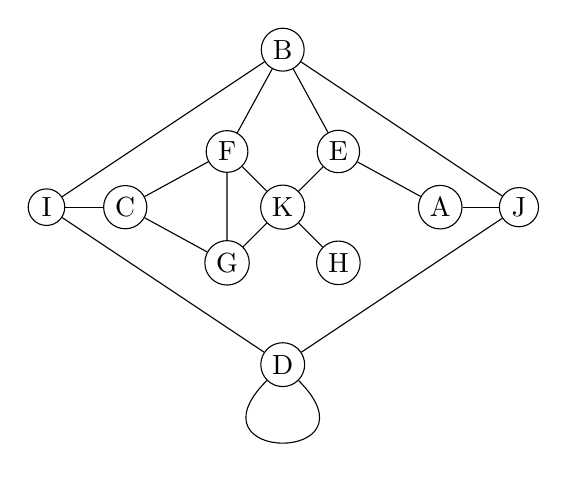
\begin{tikzpicture}[vertex/.style={circle, draw, inner sep=2pt}, every node/.style={vertex}]%, minimum size=6pt]

%\tikzstyle{every node} = [vertex];
\node (A) at (0:2) {A};
\node (B) at (90:2) {B};
\node (C) at (180:2) {C};
\node (D) at (270:2) {D};
\node (O) at (0,0){K};
\node (E) at (45:1) {E};
\node (F) at (45+90:1){F};
\node (G) at (45+180:1){G};
\node (H) at (45+270:1){H};
\node[left of = C] (I) {I};
\node [right of = A] (J) {J};
\draw (D) to[out = 270-45, in = 270+45, distance = 1.5cm] (D);
\draw (B) -- (I) -- (D) -- (J)--(B);
\draw (A) -- (E) -- (B) -- (F) -- (C) -- (G);% -- (D) -- (H) -- (A);
\draw (E) -- (O) -- (G)-- (F) --(O) --(H);
\draw (A) -- (J) (C) -- (I);
\end{tikzpicture}
%\end{minipage}
\be
%\begin{minipage}{.6\linewidth}
\item How many vertices does graph $Q$ have? \ans
\item How many edges does graph $Q$ have? \ans
\item Degree of vertex $A$? \ans
\item  Degree of vertex $H$? \ans
\item  Degree of vertex $D$? (remember, loops count twice) \ans
\item Label each vertex on the right-hand copy of the graph with its degree.
\item  Which vertex/vertices has/have the largest degree? \ans
%\end{minipage}
\item Find a path from $K$ to $D$. Draw it on the (left-hand) graph. How many edges does your path have? \ans
\item What is the length of the shortest path from $I$ to $J$? \ans Write the path here: \ans
\item Find a circuit in the graph and highlight it on the graph. Write the circuit here: \ans
\item Find a path that visits every vertex exactly once. Highlight it on the right-hand copy of the graph.

%\begin{tikzpicture}[vertex/.style={circle, draw, inner sep=1pt}, every node/.style={vertex}, scale = .8]%, minimum size=6pt]
%
%%\tikzstyle{every node} = [vertex];
%\node (A) at (0:2) {A};
%\node (B) at (90:2) {B};
%\node (C) at (180:2) {C};
%\node (D) at (270:2) {D};
%\node (O) at (0,0){K};
%\node (E) at (45:1) {E};
%\node (F) at (45+90:1){F};
%\node (G) at (45+180:1){G};
%\node (H) at (45+270:1){H};
%\node[left of = C] (I) {I};
%\node [right of = A] (J) {J};
%\draw (D) to[out = 270-45, in = 270+45, distance = 1.5cm] (D);
%\draw (B) -- (I) -- (D) -- (J)--(B);
%\draw (A) -- (E) -- (B) -- (F) -- (C) -- (G);% -- (D) -- (H) -- (A);
%\draw (E) -- (O) -- (G) (F) --(O) --(H);
%\draw (A) -- (J) (C) -- (I);
%\end{tikzpicture}
\item Explain why you can't find a circuit that passes through every vertex of the graph.

\vspace{.5in}

\item Create a context for this graph. What might the vertices represent? What might the edges represent?
\vspace{2in}
\ee

\newpage
\item Here's a second graph, Graph R.

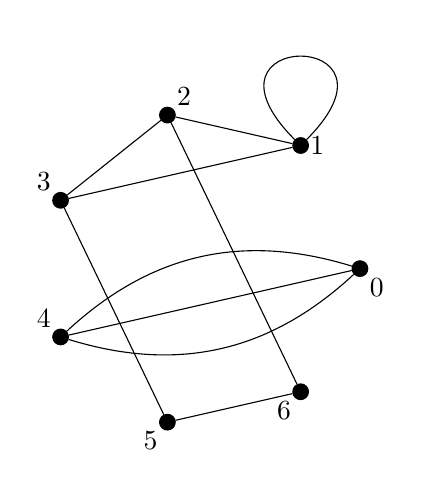
\begin{tikzpicture}[]
\foreach \i in {0, ...,6}{  \node[draw, circle, fill=black, inner sep = 2 pt, label={[label distance=-3pt]\i*360/7-50:$\i$}](\i) at (\i*360/7: 2) {};}
%\draw (1) -- (3) to[bend left = 10] node[midway, fill = white, inner sep = 1pt] {$e_{5}$}  (0);
%\draw (0)  to[bend left = 10] node[midway, fill = white, inner sep = 1pt] {$e_{4}$}  (3);
%\draw (2) to[bend right = 15] (5) -- (4) to[bend left = 10] node[midway, fill = white, inner sep = 1pt] {$e_{2}$}  (6) -- (0) --(1)--(6);
\draw (3) -- (5)--(6) -- (2) -- (3);
\draw (2) -- (1) -- (3);
\draw (0) to[bend left = 30] (4);%node[midway, fill = white, inner sep = 1pt] {$e_{1}$} (4);
\draw (0) -- (4);
\draw (0) to[bend right = 30] (4);%node[midway, fill = white, inner sep = 1pt] {$e_{3}$}  (4);
\draw (1) to[loop, distance =2cm] (1);%  node[midway, fill = white, inner sep = 1pt] {$e_{6}$} (1);
 \end{tikzpicture}
% 
%

\be
\item Explain why this graph is not connected. 

\vspace{2cm}

A \emph{connected component} is a piece of a graph that \emph{is} connected. To the right of the graph, draw the two connected components of graph R separately, with no crossing edges. (You will need to change the position of the vertices and edges!) 

\item Label each vertex with its degree.
\item How many edges does graph R have? \ans
\item Using the above graph R and the previous graph Q, fill in the following table:

{
\renewcommand{\arraystretch}{2}
\begin{tabular}{c | c | c}
Graph & sum of the degrees& number of edges\\ \hline
Graph Q &  & \\ \hline
Graph R &  & \\ \hline
\end{tabular}
}

What do you notice about the relationship between the sum of the degrees and the number of edges?\vspace{1in}

\ee

\end{enumerate}

\end{document}

%-------------------------------------------------------------------------------------------------------------------------------------------------------------------------------------------------------------------

%%% Local Variables:
%%% mode: latex
%%% TeX-master: t
%%% End:
